\documentclass[11pt, table]{beamer}
%\usepackage[table,x11names]{xcolor}
\usepackage[utf8]{inputenc}
\usepackage[T1]{fontenc}
\usepackage{multirow}
\usepackage{calc}
\usepackage{array}
\usepackage{graphicx}
\usepackage{multirow}

\newcommand{\p}{\pause}


\usetheme{default}

\newcommand\MyBox[2]{
	\fbox{\lower0.75cm
		\vbox to 1.7cm{\vfil
			\hbox to 1.7cm{\hfil\parbox{1.4cm}{#1\\#2}\hfil}
			\vfil}%
	}%
}

\begin{document}
	%\author{}
	\title{Introduction to Logistic Regression}
	%\subtitle{}
	%\logo{}
	%\institute{}
	%\date{}
	%\subject{}
	%\setbeamercovered{transparent}
	%\setbeamertemplate{navigation symbols}{}
	\begin{frame}[plain]
	\maketitle
\end{frame}

\begin{frame}
\frametitle{Logistic Regression}
\textbf{Example:} Duchenne Muscular Dystrophy (DMD)
\begin{itemize}
	\item Genetically-transmitted disease
	\item Passed from a mother to her children
	\item Female offspring suffer no apparent symptoms, but male offspring with the disease die at a young age.
	\item Female carriers tend to exhibit elevated levels of certain serum enzymes or proteins.
\end{itemize}
\vspace{0.1in}

Let's say we want to build a model which takes as input the serum levels and outputs our prediction about whether or not a female is a carrier.
\end{frame}

\begin{frame}
\frametitle{Logistic Regression}

We can start be doing some exploratory analysis.

\begin{center}
	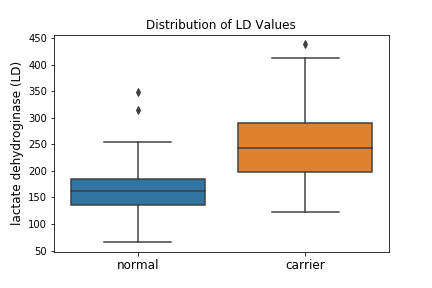
\includegraphics[width = 3in]{images/Dystrophy/LD_box.png}
\end{center}

What we can see is that in our datset, carriers tend to have higher LD values. However, there is some overlap between carriers and non-carriers in the middle values. There is not a single cutoff we can use to classify a person as a carrier or non-carrier.
\end{frame}

\begin{frame}
\frametitle{Logistic Regression}

Here is another view of the data, using a scatterplot

\begin{center}
	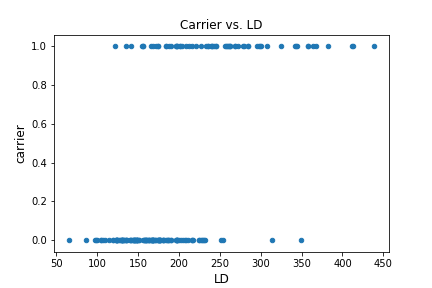
\includegraphics[width = 3in]{images/Dystrophy/scatter_01.png}
\end{center}

Here, we have encoded whether a person is a carrier or not using a numeric 0/1 value. A value of 1 indicates that a person is a carrier. 
\end{frame}


\begin{frame}
\frametitle{Logistic Regression}
Since there is overlap between carriers and non-carriers, we would probably be best off to not just make a simple prediction of carrier/non-carrier, but instead predict the likelihood or probability that a female is a carrier.
\vspace{0.1in}

From what we have seen in the plots, females with higher LD values look more likely to be carriers that those with lower values.
\vspace{0.1in}

 Between 175 and 225, it is not clear if a person is a carrier or not, so we might be best off assigning a probability close to 0.5 for people in that range.
\end{frame}

\begin{frame}
\frametitle{Logistic Regression}
So how do we create our model? We can try using a linear regression model.\p
\vspace{0.1in}

A linear regression model produces the following result:
$$\text{P(carrier)} = 0.00423\cdot(\text{LD}) - 0.4757$$

\begin{center}
	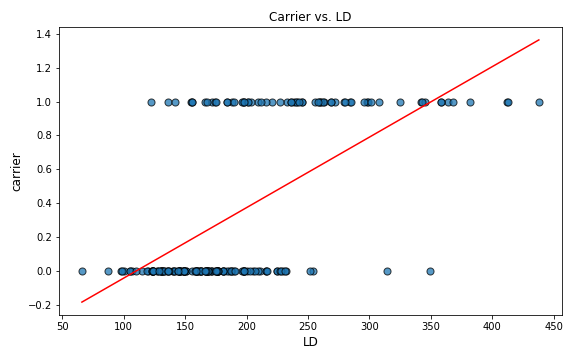
\includegraphics[width = 3in]{images/Dystrophy/scatter_02.png}
\end{center}
\end{frame}

\begin{frame}
\frametitle{Logistic Regression}
This approach has a big problem: probabilities are values between 0 and 1, but this equation has guarantee of outputting values between 0 and 1.
\vspace{0.1in}

In fact, we can see that for some values, we get predictions less than 0 or greater than 1.
\vspace{0.1in}

Another problem is that it assumes a fixed change in LD will have a fixed effect on the probability. That is, a change from 60 to 70 will have the same impact as a change from 250 to 260.
\end{frame}

\begin{frame}
\frametitle{Logistic Regression}
One possible solution to this problem is to "squash" our output between 0 and 1.
\vspace{0.1in}

A common way to do this is to pass the output from a linear model into the \textbf{logistic function}:
$$l(x) = \frac{1}{1 + e^{x}}$$

\begin{center}
	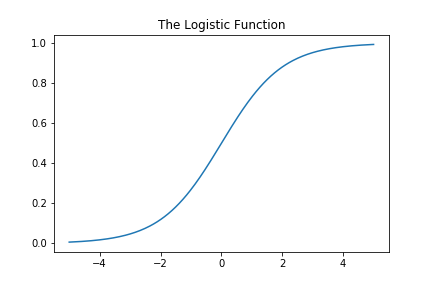
\includegraphics[width = 3in]{images/Dystrophy/logistic.png}
\end{center}
\end{frame}

\begin{frame}
\frametitle{Logistic Regression}
This means that instead of our model looking like
$$\text{P(carrier)} = \beta_1\cdot(\text{LD}) + \beta_0$$

it will look like
$$\text{P(carrier)} = \frac{1}{1 + e^{-(\beta_1\cdot(\text{LD}) + \beta_0)}}$$
\end{frame}

\begin{frame}
\frametitle{Logistic Regression}
Fitting this model, we obtain
$$\text{P(carrier)} = \frac{1}{1 + e^{-(0.0279\cdot(\text{LD}) - 6.1492)}}$$
And here are those probabilities plotted against the test set:
\begin{center}
	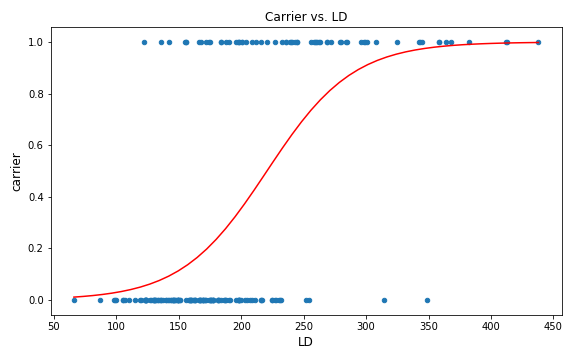
\includegraphics[width = 3in]{images/Dystrophy/scatter_03.png}
\end{center}

\end{frame}

\begin{frame}
\frametitle{Logistic Regression}
How do we assess how good our model is? 

One option is to determine how "calibrated" our model is. That is, if we look at people who we say have a 25\% probability of being a carrier, we want about 25\% of them to be carriers.
\vspace{0.1in}

Using this idea, we can build a \textbf{calibration curve}. This curve by constructed by:
\begin{enumerate}
	\item Binning the data into groups based on predicted probabilities.
	\item Computing the average predicted probability for each group.
	\item Computing the observed proportion for each group, along with a confidence interval (usually a 95\% confidence interval).
	\item Plot the observed probabilities and confidence intervals against the average probabilities for each group.
\end{enumerate}

Ideally, the plotted points should fall close to the line $y = x$ (because predicted probabilities should be similar to observed probabilities).
\end{frame}

\begin{frame}
\frametitle{Logistic Regression}
\begin{center}
	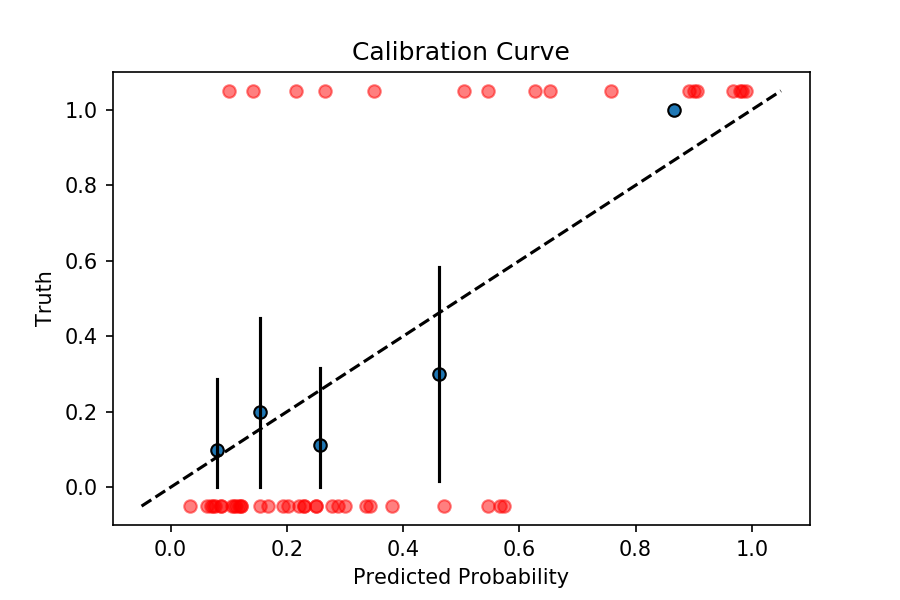
\includegraphics[width=3in]{images/Dystrophy/calib_01.png}
\end{center}

The model is decently calibrated. All of our confidence intervals intersect the line $y=x$, but the second and third point estimates are a bit low. Also, we have a smallish sample size, so we need to be cautious. 
\end{frame}

\begin{frame}
\frametitle{Logistic Regression}
Another way we could look at performance is to calculate how well our model discriminates between positive classes and negative classes. 
\vspace{0.1in}

That is, does the model tend to assign higher probabilities to positive observations compared to negative observations. 
\vspace{0.1in}

\begin{center}
	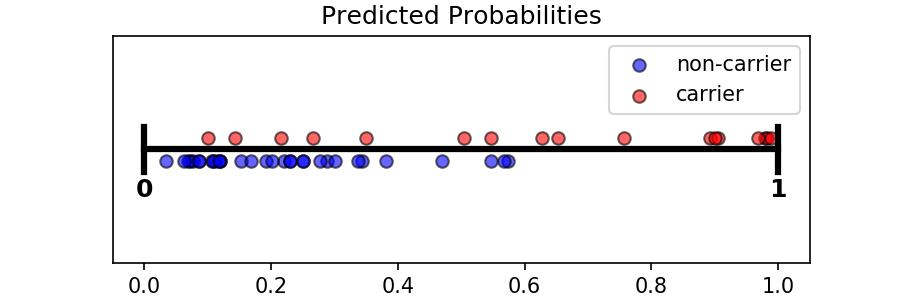
\includegraphics[width = 2.5in]{images/Dystrophy/pred_proba_01.png}
\end{center}
\end{frame}

\begin{frame}
\frametitle{Logistic Regression}
Closely related to the plot of the predicted probabilities is the Receiver Operator Characteristic Curve (ROC).

\begin{center}
	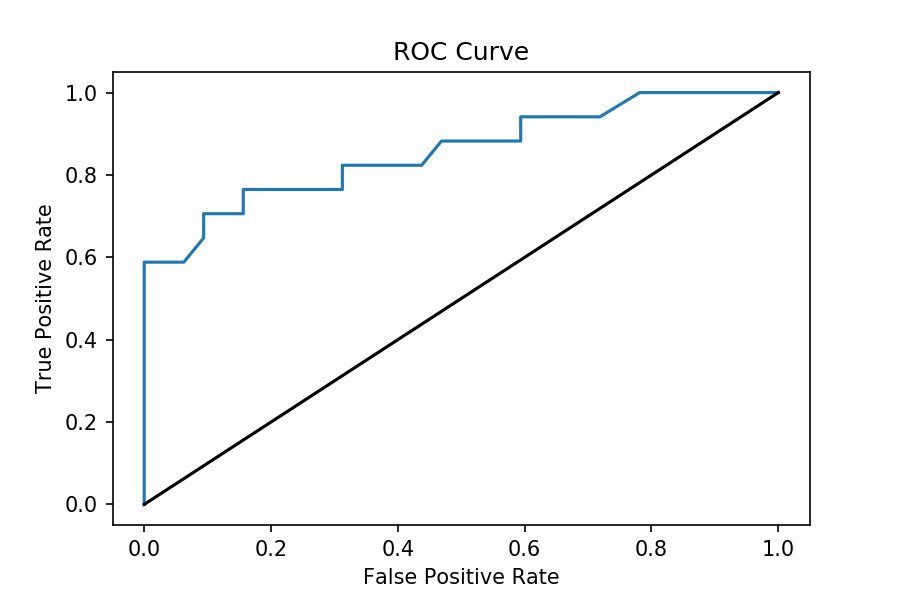
\includegraphics[width = 2.5in]{images/Dystrophy/roc_01.png}
\end{center}

This curve shows the tradeoff between correctly classifying those who are carriers vs. incorrectly classifying those who are not carriers as we adjust the threshold for how sure we have to be to predict that a person is a carrier (see demonstration).
\end{frame}

\begin{frame}
\frametitle{Logistic Regression}
\begin{center}
	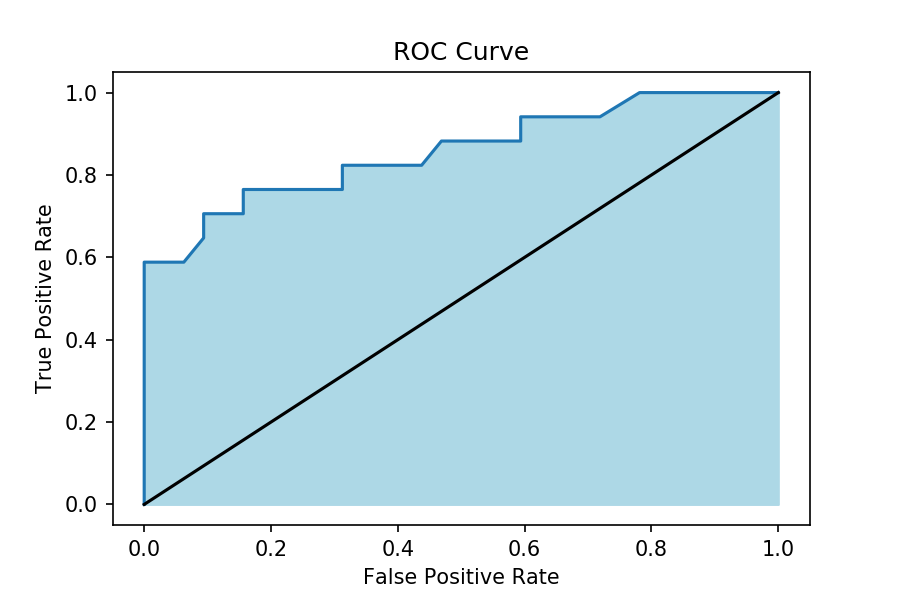
\includegraphics[width = 2.5in]{images/Dystrophy/roc_02.png}
\end{center}

The Area under the Receiver Operater Characteristic Curve (ROC AUC) is a useful metric to see how well the model discriminates between the positive and negative classes.
\vspace{0.1in}

This area is the same as the probability that, given a random positive and a random negative observation, the model assigns a higher probability to the positive observation. 
\end{frame}

\begin{frame}
\frametitle{Logistic Regression}
\begin{center}
	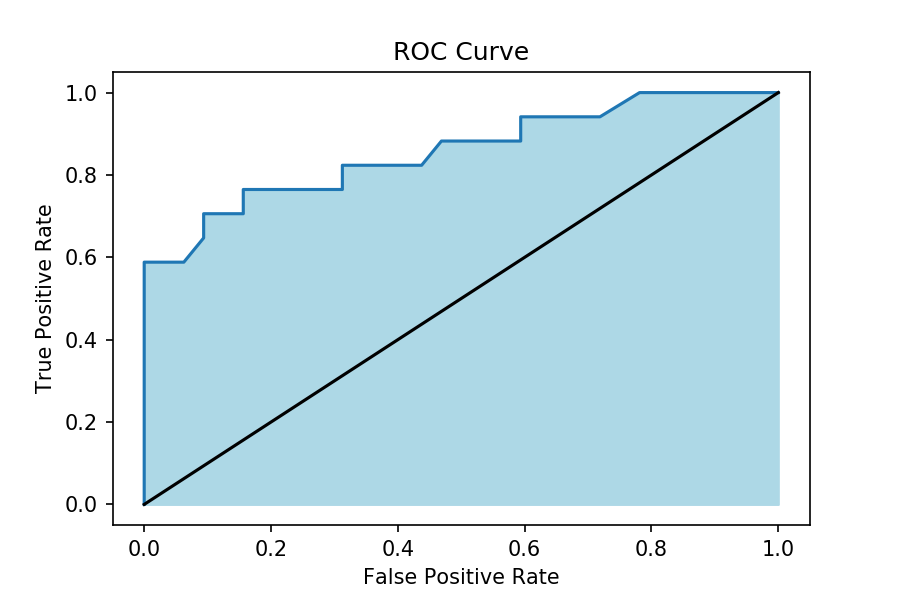
\includegraphics[width = 2.5in]{images/Dystrophy/roc_02.png}
\end{center}

Here, the area under the curve is 0.8539.

\end{frame}

\begin{frame}
\frametitle{Logistic Regression}
The last thing to do is to assign predictions based on probabilities. The normal convention would be to predict that anyone with a predicted probability greater than 0.5 is a carrier and everyone else as a non-carrier. If we do this, we get the following results on the test set:

\begin{center}
	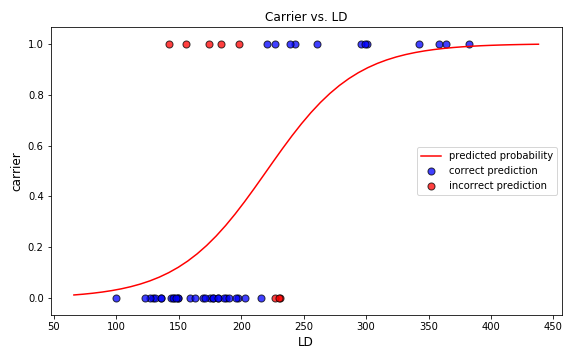
\includegraphics[width = 3in]{images/Dystrophy/scatter_04.png}
\end{center}

\end{frame}

\begin{frame}
\frametitle{Logistic Regression}
There are two type of wrong predictions:\p
\begin{itemize}
	\item Non-carriers who were predicted as being carriers (\textbf{False Positives})\p
	\item Carriers who were predicted as not being carriers (\textbf{False Negatives})\p
\end{itemize}
We can organize all of the cases into a \textbf{confusion matrix}:

\begin{center}
	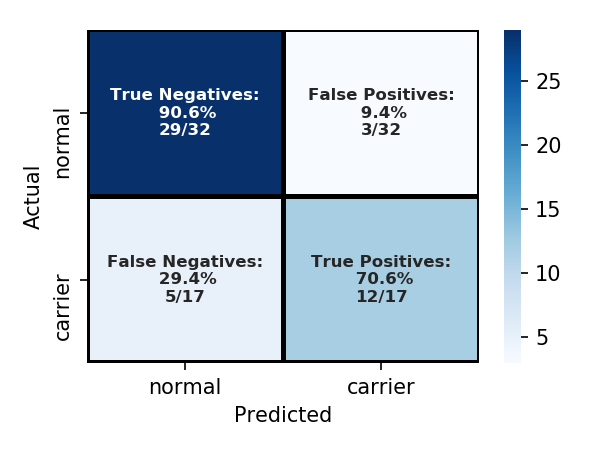
\includegraphics[width=2.5in]{images/Dystrophy/cm.png}
\end{center}
\end{frame}

\begin{frame}
\frametitle{Logistic Regression}
How might we try and improve our model?
\vspace{0.1in}

We have three other serum values in our datset, so we could add those in as additional predictor variables. This will turn our model into one that looks like

$$P(carrier) = \frac{1}{1 + e^{-(\beta_0 + \beta_1\cdot(\text{CK}) + \beta_2\cdot(\text{H}) + \beta_3\cdot(\text{PK}) + \beta_4\cdot(\text{LD}))}}$$
\end{frame}

\begin{frame}
\frametitle{Logistic Regression}
After fitting the model, we get

$$P(carrier) = \frac{1}{1 + e^{-(-17.2254 + 0.0446(\text{CK}) + 0.1163(\text{H}) + 0.0875(\text{PK}) + 0.0122(\text{LD}))}}$$
\end{frame}

\begin{frame}
\frametitle{Logistic Regression}
\begin{center}
	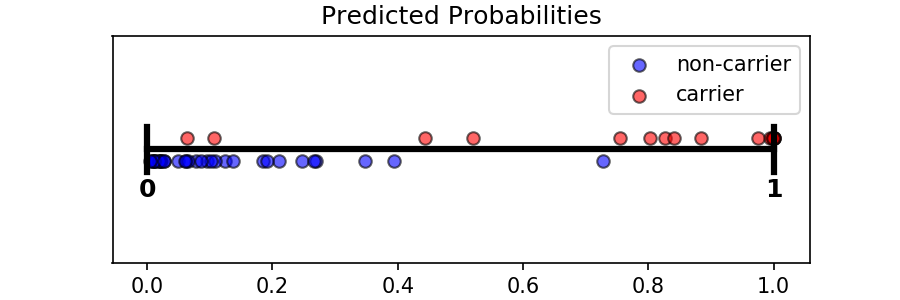
\includegraphics[width=2.5in]{images/Dystrophy/pred_proba_02.png}
\end{center}

\begin{center}
	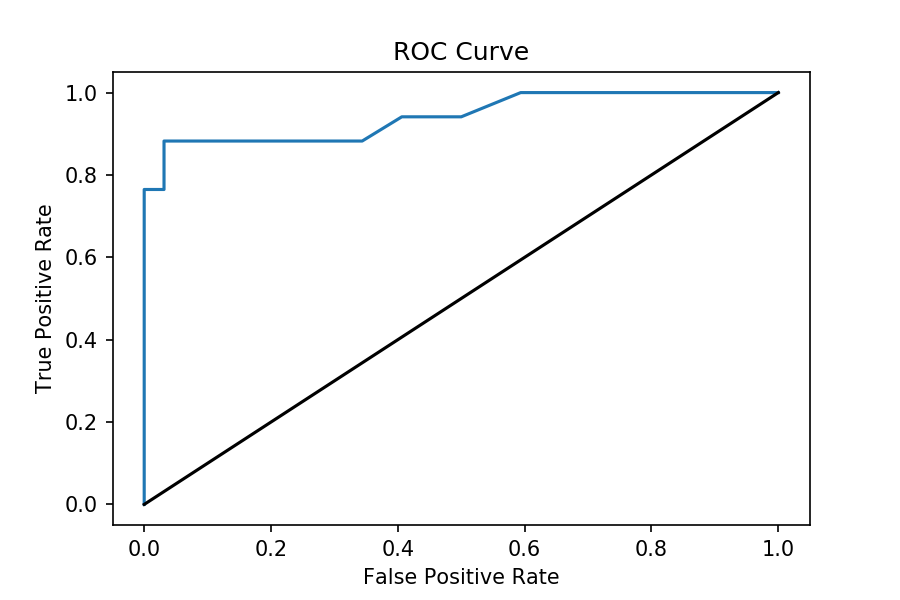
\includegraphics[width=2.5in]{images/Dystrophy/roc_03.png}
\end{center}
\end{frame}

\begin{frame}
\frametitle{Logistic Regression}
\begin{center}
	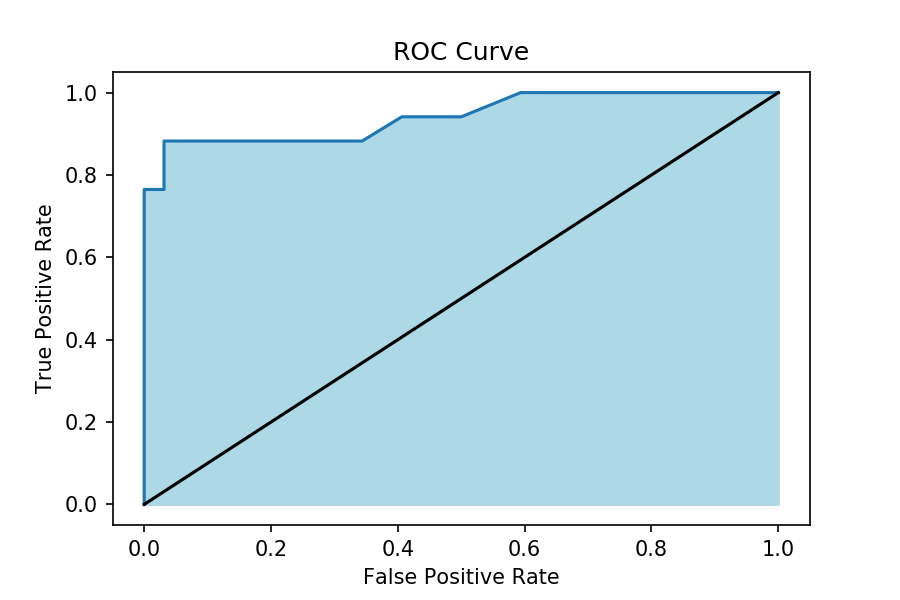
\includegraphics[width=2.5in]{images/Dystrophy/roc_04.png}
\end{center}

This time, the area under the curve is 0.9430.
\end{frame}

\begin{frame}
\frametitle{Logistic Regression}
Using this model, we see a higher percentage of correct predictions.

\begin{center}
	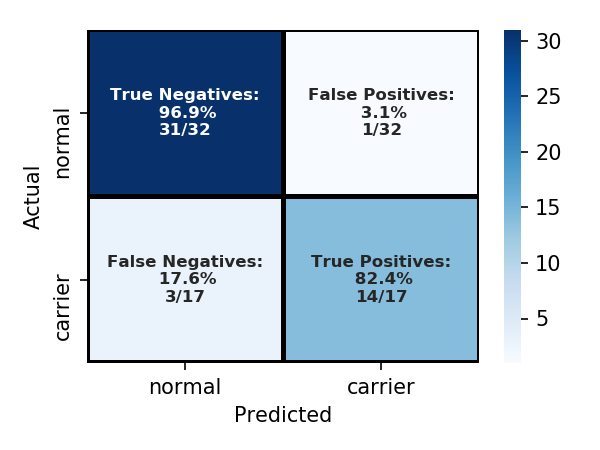
\includegraphics[width=2.5in]{images/Dystrophy/cm_2.png}
\end{center}

\end{frame}

\end{document}
